\documentclass{beamer}
\usetheme{metropolis}

\usepackage[ngerman]{babel}
\usepackage[autostyle=true,german=quotes]{csquotes}
\usepackage[linewidth=1pt]{mdframed}
\usepackage{hyperref}
\usepackage{makecell}
\usepackage{pifont}
\usepackage{tikz}
\usetikzlibrary{positioning, calc, arrows, fit, decorations.pathreplacing, shapes, shapes.multipart, snakes}
\usepackage{verbatim}
\usepackage{textcomp}
%\usepackage{pdfpages}

\batchmode

\hypersetup{
	colorlinks,
	urlcolor=blue,
	linkcolor=black % for ToC
}
\newenvironment{qaa}[1]{
	#1

	\begin{mdframed}
		\small
}{
	\end{mdframed}
}

\newcommand{\true}{\ding{51}}
\newcommand{\false}{\ding{55}}
\newcommand{\code}[1]{
	\begin{mdframed}
		\verbatiminput{#1}
	\end{mdframed}
}

\title{Tutorium 04: Entwurf in Haskell}
% \subtitle{}
\author{Paul Brinkmeier}
\institute{Tutorium Programmierparadigmen am KIT}
\date{12. November 2019}

\begin{document}

\begin{frame}
	\titlepage
\end{frame}

\section{Heutiges Programm}
\begin{frame}{Programm}
	\begin{itemize}
		\item Übungsblatt 3
		\item Software-Entwurf in Haskell
	\end{itemize}
\end{frame}

\section{Übungsblatt 3}

\begin{frame}{1 --- Streams}
	\code{demos/Fibs.hs}

	\begin{itemize}
		\item Schön kompakt
		\item \texttt{zipWith} ist endrekursiv $\Rightarrow$ linearer Speicher 
		\item \texttt{fibs !! n} $\in O($\pause$n)$
		\begin{itemize}
			\item (wenn Addition konstant)
		\end{itemize}
	\end{itemize}
\end{frame}

\begin{frame}{2 --- Collatz-Vermutung}
	\code{demos/Collatz.hs}
\end{frame}

\begin{frame}{2 --- Collatz-Vermutung}
	\code{demos/CollatzAlt.hs}

	\begin{itemize}
		\item \enquote{eleganter}
		\item In der Klausur aber eher nur Funktionen aus der Prelude verwenden
	\end{itemize}
\end{frame}

\begin{frame}{3 --- Stream-Kombinatoren}
	\code{demos/Merge.hs}

	\begin{itemize}
		\item Für \texttt{i} in \texttt{1..n} unendliche Liste der Primzahlen hoch \texttt{i} erstellen
		\item Wegen Laziness: wird nur so weit ausgewertet wie nötig
		\item Dann: Alle miteinander vereinigen
	\end{itemize}
\end{frame}

\begin{frame}{\texttt{:sprint}}
	\code{code/ghci-sprint.output}

	\begin{itemize}
		\item \texttt{:sprint a} gibt aktuelle Speicherrepräsentation für \texttt{a} aus
		\item \texttt{\_} steht dabei für \enquote{noch nicht ausgewertet}
		\item $\leadsto$ praktisch für Debugging unendlicher Listen
	\end{itemize}
\end{frame}

\section{Wiederholung: Algebraische Datentypen}

\begin{frame}{Algebraische Datentypen}
	\code{demos/DataExamples.hs}

	\begin{itemize}
		\item Keyword \text{data} definiert \emph{neuen} Typ
		\item \enquote{\texttt{enum} auf Meth}
		\item Ersetzt oft Vererbung im Entwurfsprozess
	\end{itemize}
\end{frame}

\section{Software-Entwurf in Haskell}

\begin{frame}{Software-Entwurf in Haskell}
	\begin{itemize}
		\item Statt abstrakter Klasse + Unterklassen: ein Summentyp
		\begin{itemize}
			\item OOP: \pause
			\begin{itemize}
				\item \texttt{abstract class Auto \{ ... \}}
				\item \texttt{class Verbrenner extends Auto \{ ... \}}
				\item \texttt{class Elektro extends Auto \{ ... \}}
			\end{itemize}
			\item FP: \pause\texttt{data Auto = Verbrenner ... | Elektro ...}
		\end{itemize}
		\item Implementierung der verschiedenen Verhaltensweisen:
		\begin{itemize}
			\item OOP: \pause\texttt{@Override void accelerate()} in Unterklassen
			\item FP: \pause\texttt{accelerate :: Auto -> Auto}, Pattern-Matching auf Varianten
		\end{itemize}
	\end{itemize}
\end{frame}

\subsection{Spielkarten}

\begin{frame}{Aufgaben: Spielkarten}
	\begin{figure}
		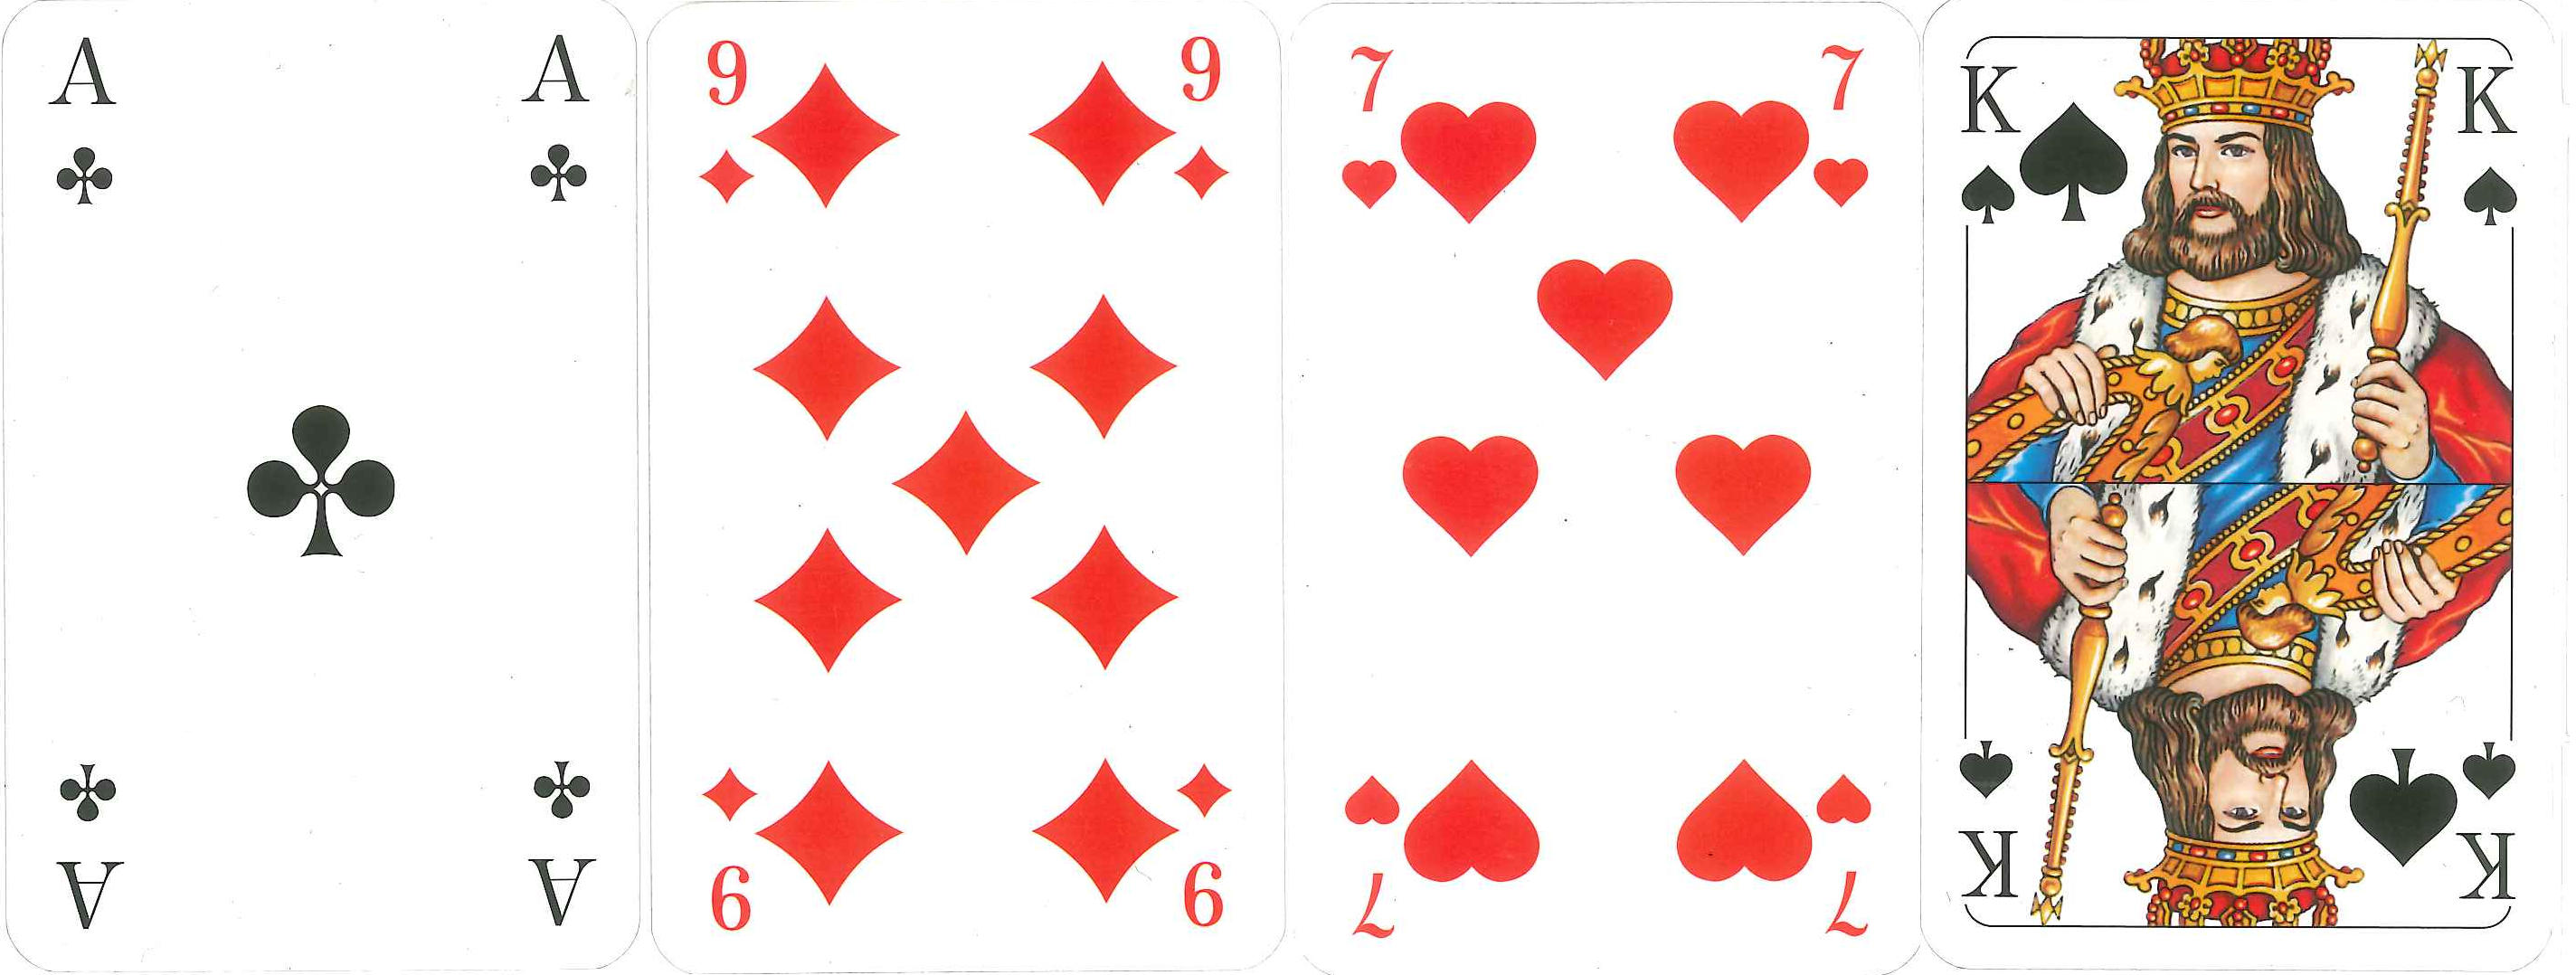
\includegraphics[width=\textwidth]{images/playing-cards}
	\end{figure}

	\code{demos/PlayingCards.hs}
\end{frame}

\begin{frame}{Aufgaben: Spielkarten}
	\code{demos/PlayingCards.hs}

	\begin{itemize}
		\item \url{//github.com/pbrinkmeier/pp-tut}
		\item Implementiert \texttt{Eq} und \texttt{Ord} für \texttt{Card}, \texttt{Suit} und \texttt{Rank}:
		\begin{itemize}
			\item \texttt{instance Eq Suit where}\\\texttt{  Spades == Spades = True}\\\texttt{  ...}
			\item Tipp für \texttt{Ord}: Abbilden auf \texttt{Int}, dann vergleichen
		\end{itemize}
		\pause
		\item Implementiert \texttt{Show} für \texttt{Card}, \texttt{Suit} und \texttt{Rank}:
		\begin{itemize}
			\item \texttt{show \$ Card Ace Spades == "{}ace of spades"{}}
			\item \texttt{show \$ Card Nine Clubs == "{}9 of clubs"{}}
		\end{itemize}
	\end{itemize}
\end{frame}

\begin{frame}{\texttt{deriving}}
	\code{demos/PlayingCards2.hs}

	\begin{itemize}
		\item Selbstimplementierung ist unnötige Schreibarbeit $\leadsto$ kann i.d.R. vom Compiler übernommen werden
		\item \texttt{deriving} funktioniert nur für \texttt{Eq}, \texttt{Ord}, \texttt{Enum}, \texttt{Enum}, \texttt{Bounded}, \texttt{Show} und \texttt{Read}
		\item Über Umwege kann man auch eigene Typklassen \texttt{derive}n, ist aber viel Aufwand
	\end{itemize}
\end{frame}

\subsection{Monopoly-Karten}

\begin{frame}{Aufgaben: Monopoly-Karten}
	\begin{figure}
		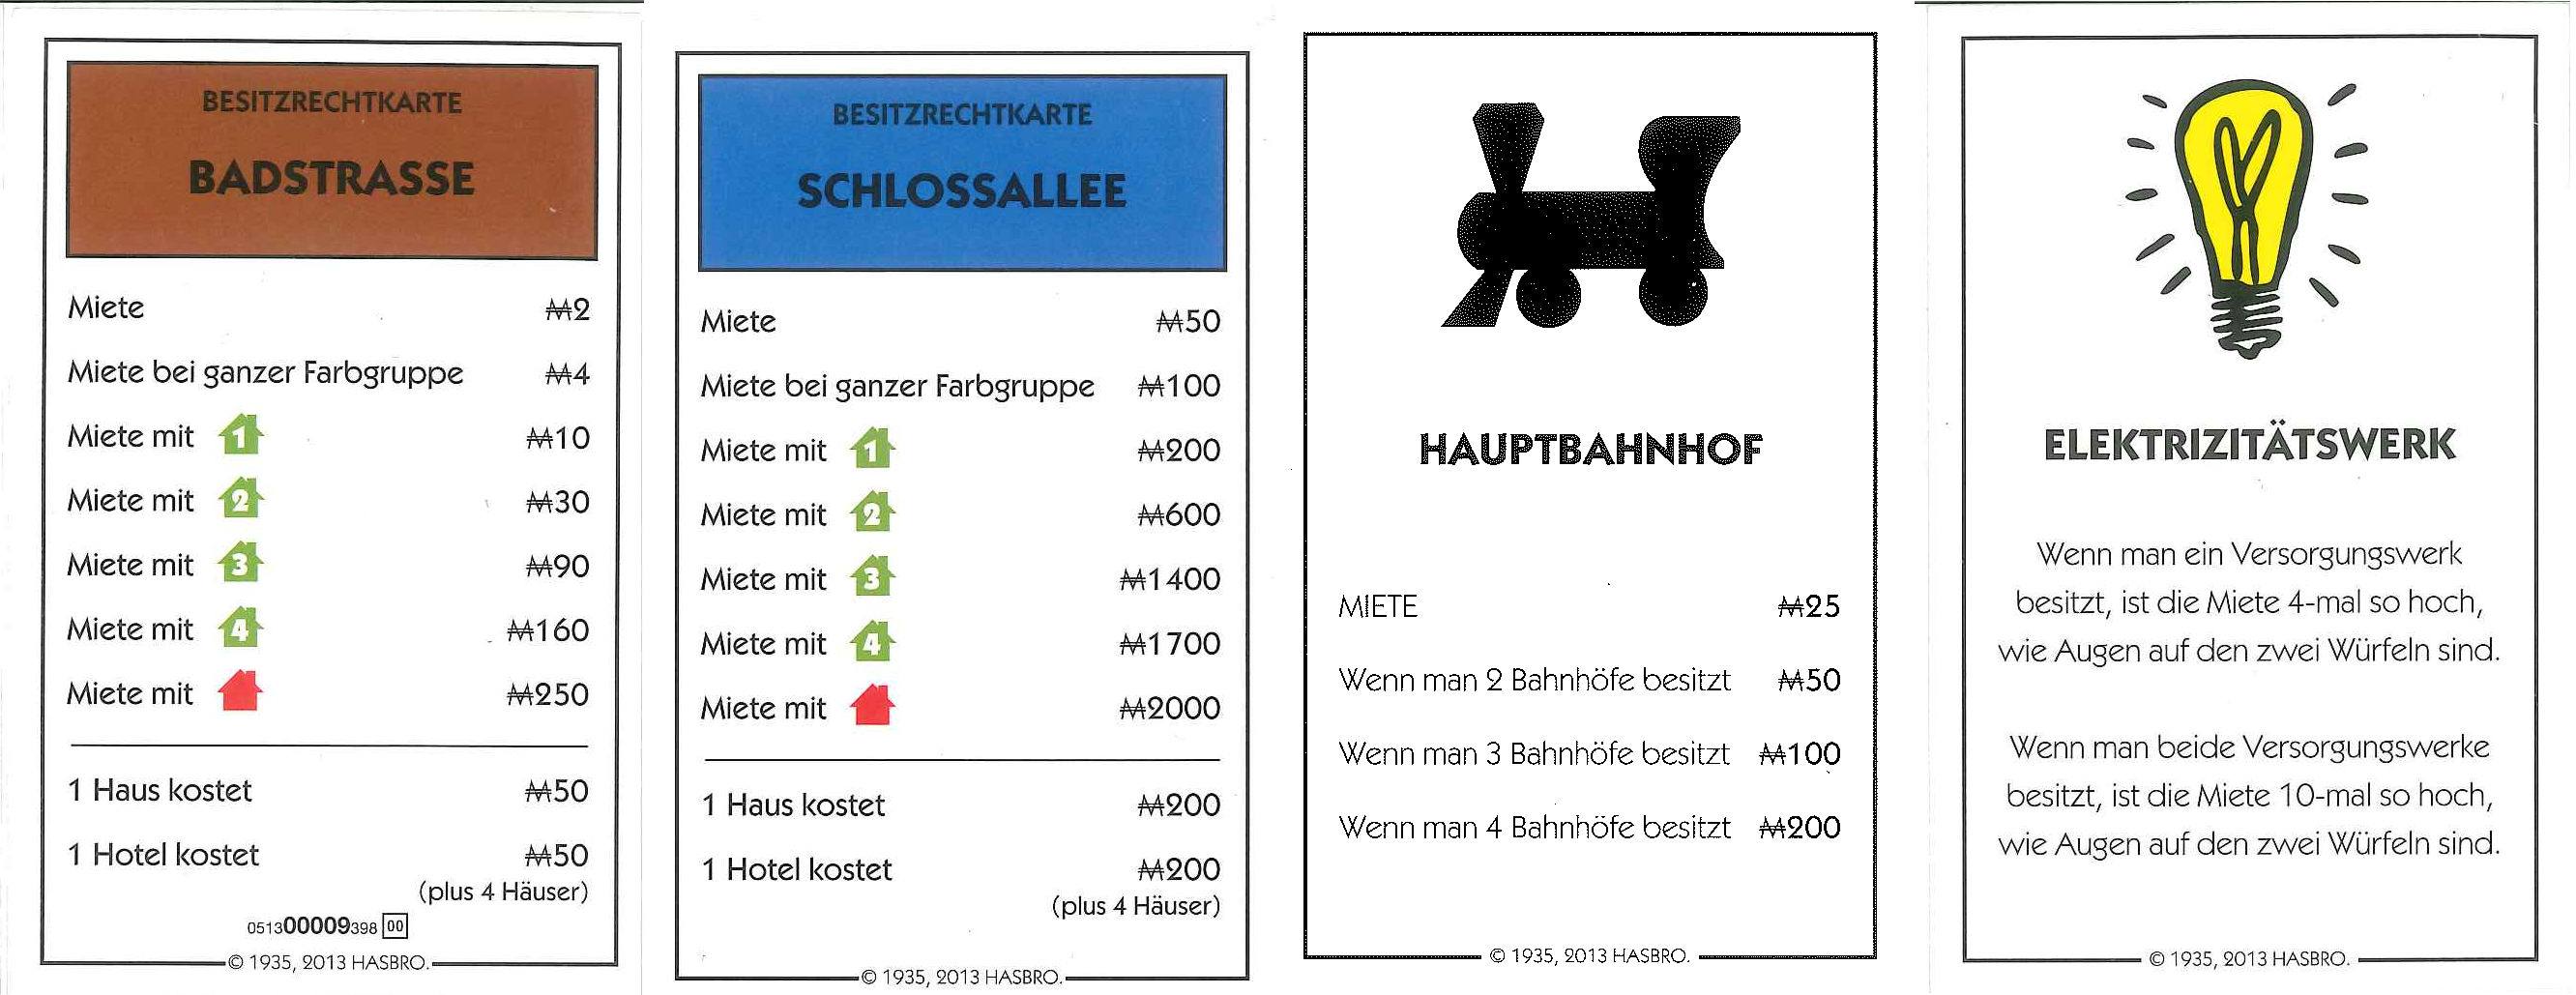
\includegraphics[width=\textwidth]{images/monopoly-cards}
	\end{figure}

	\code{demos/MonopolyCards.hs}
\end{frame}

\begin{frame}{Aufgaben: Monopoly-Karten}
	\code{demos/MonopolyCards.hs}

	\begin{itemize}
		\item Sagt dem Compiler, dass \texttt{Card} vergleich- und sortierbar ist
		\item Implementiert \texttt{Show Card}:
		\begin{itemize}
			\item \texttt{show badStrasse == "{}Str (braun) Badstrasse: Haus = 50M"{}}
			\item \texttt{show hauptbahnhof == "{}Sta Hauptbahnhof"{}}
			\item \texttt{show electricCompany == "{}Utl Elekritzitätswerk"{}}
		\end{itemize}
	\end{itemize}
\end{frame}

\begin{frame}{Aufgaben: Monopoly-Karten}
	\code{demos/MonopolyRent.hs}

	\begin{itemize}
		\item Schreibt eine Funktion, die die Miete eines Felds ausrechnet
		\item Die Funktion nimmt:
		\begin{itemize}
			\item Die Karte, auf der man gelandet ist
			\item Die Liste der Karten des Besitzers (für bspw. Bahnhöfe)
			\item Die Summe der Augen, die gewürfelt wurden (für die Werke)
		\end{itemize}
		\item Die Funktion soll die Miete als \texttt{Int} zurückgeben
	\end{itemize}
\end{frame}

\end{document}
